\documentclass[11pt]{article}

% --- PACKAGES ---
\usepackage[utf8]{inputenc}
\usepackage[T1]{fontenc}
\usepackage{amsmath}
\usepackage{amssymb}
\usepackage{geometry} % Loaded geometry
\usepackage[pdftex,pdfpagelabels,bookmarks,hyperindex,hyperfigures]{hyperref} % hidelinks removed for colorlinks
\usepackage{authblk}
\usepackage{tikz} % For drawing the diagram
\usepackage{booktabs}   % For professional-looking tables
\usepackage{array}      % For cell padding in tables
\usepackage{float}      % For more precise float placement [H]
\usepackage{amsthm}     % For theorem-like environments (definition, proposition)
% \usepackage{orcidlink} % For ORCID iD - Replaced with \thanks

% --- CUSTOMIZATIONS ---
\geometry{margin=1in} % Set margin as per arXiv default
\renewcommand{\arraystretch}{1.5} % Increases vertical padding in tables
\newcommand{\GB}[2]{\bigl(#1,#2\bigr)} % Macro for (G,B) pairs

\newtheorem{definition}{Definition}[section]
\newtheorem{proposition}{Proposition}[section]
\newtheorem{lemma}{Lemma}[section]
\newtheorem{theorem}{Theorem}[section]
\newtheorem{corollary}{Corollary}[section]
\theoremstyle{remark} 
\newtheorem{example}{Example}[section]

% --- DOCUMENT INFORMATION ---
\title{Good/Bad (G-B) Logic: A Foundational Sketch}
\author{Brian Searls\thanks{ORCID: 0009-0002-9804-0731}} % ORCID via \thanks, standard hyphenation
\date{\today}

% --- PDF METADATA AND HYPERREF COLORS ---
\makeatletter
\hypersetup{
    pdftitle={Good/Bad (G-B) Logic: A Foundational Sketch},
    pdfauthor={Brian Searls},
    pdfsubject={cs.LO, math.LO}, % Added math.LO as secondary
    pdfkeywords={{Multi-valued logic},{Paraconsistent logic},{Knowledge representation},{Logical foundations},{Emergent semantics},{Bipolar logic}}, % Condensed & sentence case keywords, with braces
    colorlinks=true, % Added for colored links
    linkcolor=blue,
    citecolor=blue,
    urlcolor=blue
}
\makeatother

% --- BEGIN DOCUMENT ---
\begin{document}

\maketitle

% --- ABSTRACT ---
\begin{abstract}
Classical bivalent logic struggles with ambiguity and conflicting information. This paper introduces Good/Bad (G-B) logic, a multi-valued system where propositions are evaluated using two independent real values in $[0,1]$: a 'Degree of Affirmation' (G) and a 'Degree of Refutation' (B). We formalize one specific instantiation of G-B logic, defining semantics for core propositional connectives ($\neg, \land, \lor, \rightarrow$) based on $\min$ and $\max$ operations. This system is paraconsistent, offers a nuanced interpretation of classical tautologies like the Law of the Excluded Middle, and, crucially, classical logic emerges as a well-defined limiting case when G/B valuations are restricted to their extremes (e.g., G$\ge 1-\varepsilon$ \& B$\le\varepsilon$ for small $\varepsilon > 0$). G-B logic provides a formal pathway for representing evaluative bipolarity, serving as a basis for reasoning under ambiguity.
\end{abstract}

\textbf{Keywords:} Multi-valued logic, Paraconsistent logic, Knowledge representation, Logical foundations, Emergent semantics, Bipolar logic

\tableofcontents
\newpage

% --- SECTION 1: INTRODUCTION ---
\section{Introduction}

\subsection{Background and Motivation}
Classical bivalent logic, with its definitive true/false evaluations, forms an indispensable cornerstone for disciplines demanding precision and unambiguous reasoning, such as formal mathematics and many areas of engineering \cite{boole1854}. Its power in these well-defined domains is undeniable. However, when applied to problem spaces characterized by inherent ambiguity, conflicting information, or nuanced subjective assessments (e.g., ethical dilemmas, human cognition, complex real-world systems), the very features that lend bivalent logic its strength—its insistence on sharp distinctions and binary outcomes—can lead to challenges. It is not that classical logic fundamentally fails in these contexts, but rather its application can lead to significant dissonance when attempting to map inherently non-binary phenomena onto its bivalent structure. Forcing such a mapping often requires an extensive proliferation of granular categories to maintain precision, leading to escalating combinatorial complexity in the representation, which can obscure underlying patterns and become unwieldy. This contrasts with the human cognitive ability to form holistic, generalized assessments of concepts without needing to explicitly process an exhaustive list of their constituent bivalent properties. 

Furthermore, classical logic's application often relies on implicitly shared contexts and definitions. Yet, the interpretation and perceived ``truth'' of many concepts are deeply intersubjective and context-dependent. Bivalent systems can struggle to make these contextual dependencies explicit and manage the resulting variations in meaning gracefully.

The G-B (Good/Bad) logical framework proposed herein is motivated by an epistemological perspective: that classical bivalent logic itself may be an \textbf{emergent property derived from more basic, bipolar evaluative mechanisms}. Such mechanisms can be observed in simple orienting systems, for instance, in the capacity to differentiate between ``good'' and ``bad'' stimuli as a foundational step for environmental interaction. This paper explores one formal instantiation of a logic grounded directly in these 'Goodness' (G) and 'Badness' (B) dimensions. Our central aim is to demonstrate how a system built on these evaluative primitives can give rise to coherent logical operations and, under specific conditions (evaluations at their extremes), yield classical bivalent logic as an emergent special case. While a comprehensive demonstration of a direct scientific link to biology or cognitive science is beyond this initial sketch and requires further interdisciplinary research, this perspective provides the fundamental motivation for the G-B framework's design.

\subsection{The G-B Valuation Proposal}
Building upon the motivating perspective that formal logic can emerge from foundational bipolar evaluations, the G-B logical framework departs from traditional single-valued truth assignments. Instead, each proposition $p$ is evaluated through an ordered pair, $V(p) = \GB{G(p)}{B(p)}$. For the foundational development in this paper, $G(p)$ represents the \textbf{Degree of Affirmation} associated with $p$, while $B(p)$ represents its \textbf{Degree of Refutation}. These G and B values are independent real numbers within the range $[0,1]$. (While the G-B Logic moniker uses ``Good/Bad'' for intuitive appeal and to acknowledge its capacity for broader evaluative applications, ``Affirmation/Refutation'' serves as the primary interpretation for the formal logical system detailed herein.)

This dual-component valuation defines a G-B space, typically visualized as the unit square, where the G-axis represents the Degree of Affirmation and the B-axis the Degree of Refutation (see Figure \ref{fig:gb_valuation_space}). Key points include:
\begin{itemize}
    \item \textbf{$\GB{1}{0}$:} Corresponds to Classical True.
    \item \textbf{$\GB{0}{1}$:} Corresponds to Classical False.
    \item \textbf{$\GB{1}{1}$:} Represents Maximal Dissonance.
    \item \textbf{$\GB{0}{0}$:} Represents Neutrality or Irrelevance.
    \item \textbf{$\GB{0.5}{0.5}$:} Signifies Ambiguity or moderate dissonance.
    \item \textbf{$\GB{0.9}{0.2}$:} An example of a state that is mostly affirmed with slight refutation (labeled ``Mostly G'').
    \item \textbf{$\GB{0.2}{0.9}$:} An example of a state that is slightly affirmed but significantly refuted (labeled ``Mostly B'').
\end{itemize}
The independence of G and B allows direct modeling of situations where positive and negative aspects coexist, addressing combinatorial overload by enabling a compact representation of multifaceted states.

\subsection{Contribution and Scope of This Paper}
The primary contribution is a \textbf{foundational sketch of one specific instantiation} of G-B propositional logic, illustrating a plausible formal pathway for classical logic's emergence from dual evaluative dimensions. This paper does not claim to establish a universally predominant G-B logic, but rather offers a robust foundational example.

The specific goals are:
\begin{itemize}
    \item To outline the epistemological motivation and clarify the interpretation of 'Degree of Affirmation' (G) and 'Degree of Refutation' (B).
    \item To define the syntax for this G-B propositional language.
    \item To detail the semantics for core logical connectives ($\neg, \land, \lor, \rightarrow$) for this instantiation.
    \item To discuss basic formal properties, including paraconsistency and its relationship to classical logic.
\end{itemize}
This paper does \textit{not} provide a full proof theory, extend to first-order logic, or formalize 'Context (C)'. Its purpose is to formalize basic G-B operations and interpretations as groundwork for further exploration.

\subsection{Structure of the Paper}
Section 2 introduces the G-B propositional framework. Section 3 provides semantic definitions for connectives. Section 4 explores formal properties and relations to other logics. Section 5 discusses this instantiation. Section 6 concludes.

% --- SECTION 2: THE G-B PROPOSITIONAL LANGUAGE AND VALUATIONS ---
\section{The G-B Propositional Language and Valuations}

\subsection{Syntax}
The G-B logic employs a standard propositional language.
\begin{definition}[Propositional Variables]
The basic elements are propositional variables from a countably infinite set, $\mathcal{P} = \{p, q, r, p_1, p_2, \dots\}$.
\end{definition}

\begin{definition}[Logical Connectives]
The primitive connectives are: $\neg$ (negation), $\land$ (conjunction), and $\lor$ (disjunction). The connective $\rightarrow$ (implication) is defined as $p \rightarrow q \equiv \neg p \lor q$.
\end{definition}

\begin{definition}[Well-Formed Formulas (WFFs)] \label{def:wff}
The set of well-formed formulas (WFFs) of the G-B propositional language is defined recursively as follows: 
\begin{enumerate}
    \item Any propositional variable $s \in \mathcal{P}$ is a WFF.
    \item If $\phi$ is a WFF, then $(\neg \phi)$ is a WFF.
    \item If $\phi$ and $\psi$ are WFFs, then $(\phi \land \psi)$ is a WFF.
    \item If $\phi$ and $\psi$ are WFFs, then $(\phi \lor \psi)$ is a WFF.
\end{enumerate}
Formulas involving the defined connective $\rightarrow$ are also considered WFFs by virtue of their definition in terms of $\neg$ and $\lor$. Parentheses are used to ensure clarity and disambiguate the scope of connectives; some may be omitted based on standard operator precedence rules where no ambiguity arises.
\end{definition}

\subsection{G-B Valuations}
\begin{definition}[G-B Valuation Function] \label{def:gb_valuation}
A G-B \textbf{valuation function}, V, assigns to each WFF $\phi$, within a given \textbf{context} C, an ordered pair:
$$V(\phi|C) \;= \GB{G(\phi|C)}{B(\phi|C)}$$ % Added \; for spacing
where $G(\phi|C) \in [0,1]$ and $B(\phi|C) \in [0,1]$.
\begin{itemize}
    \item $G(\phi|C)$ is the \textbf{Degree of Affirmation} of $\phi$ in context C.
    \item $B(\phi|C)$ is the \textbf{Degree of Refutation} of $\phi$ in context C.
\end{itemize}
\end{definition}
The underlying principle is that many forms of evaluation involve distinguishing between two opposing poles. The G-B framework provides a structure for such bipolar assessments, with the specific meaning of 'Affirmation' and 'Refutation' being established through intersubjective agreement within context C. The assignment of initial pairs $\GB{G}{B}$ (chosen in context $C$) to atomic propositions is fundamentally shaped by C. For example, $p \equiv \text{``The Earth is round.''}$: % Corrected grammar
\begin{itemize}
    \item In context $C_1$ (modern science): $V(p|C_1) \approx \GB{1.0}{0.0}$.
    \item In context $C_2$ (ancient flat-Earth belief): $V(p|C_2) \approx \GB{0.1}{0.9}$.
\end{itemize}
Logical operations in Section 3 assume a consistent context C. For brevity in the formulas that follow, $G(\phi|C)$ and $B(\phi|C)$ will be denoted $G_\phi$ and $B_\phi$ respectively (context C being implicit unless specified). The formalization of Context (C) itself is beyond the scope of this foundational sketch.

\begin{figure}[H]
\centering
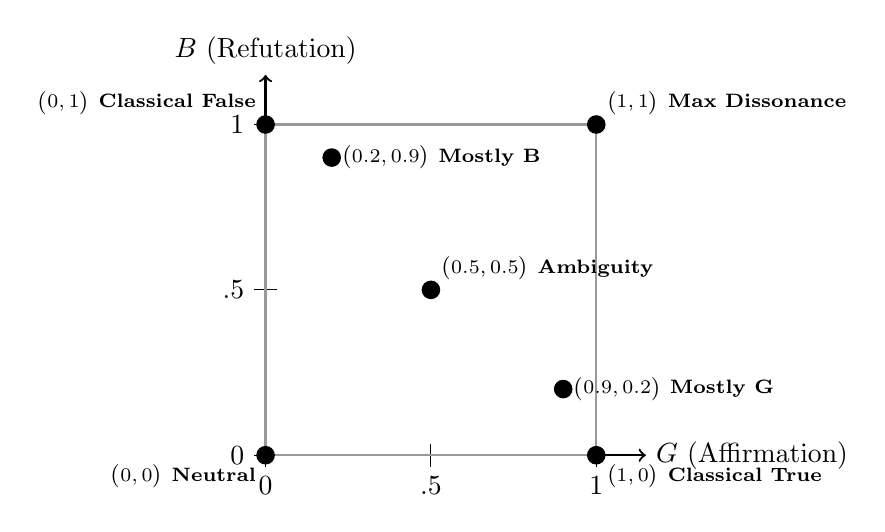
\begin{tikzpicture}[scale=4.2] % Adjusted scale
  \draw[->,thick] (0,0)--(1.15,0) node[anchor=west]{\(G\) (Affirmation)};
  \draw[->,thick] (0,0)--(0,1.15) node[anchor=south]{\(B\) (Refutation)};
  \foreach \x in {0,.5,1} \draw(\x,1pt)--(\x,-1pt) node[anchor=north]{\(\x\)};
  \foreach \y in {0,.5,1} \draw(1pt,\y)--(-1pt,\y) node[anchor=east]{\(\y\)};
  \draw[gray!80,thick](0,0) rectangle (1,1);
  \fill(1,0) circle(.8pt) node[below right,font=\scriptsize\bfseries]{$\GB{1}{0}$ Classical True}; % Adjusted font
  \fill(0,1) circle(.8pt) node[above left,font=\scriptsize\bfseries]{$\GB{0}{1}$ Classical False}; % Adjusted font
  \fill(1,1) circle(.8pt) node[above right,font=\scriptsize\bfseries]{$\GB{1}{1}$ Max Dissonance}; % Adjusted font
  \fill(0,0) circle(.8pt) node[below left,font=\scriptsize\bfseries]{$\GB{0}{0}$ Neutral}; % Adjusted font
  \fill(.5,.5) circle(.8pt) node[above right,font=\scriptsize\bfseries]{$\GB{0.5}{0.5}$ Ambiguity}; % Adjusted font
  \fill(.9,.2) circle(.8pt) node[right,font=\scriptsize\bfseries]{$\GB{0.9}{0.2}$ Mostly G}; % Adjusted font
  \fill(.2,.9) circle(.8pt) node[right,font=\scriptsize\bfseries]{$\GB{0.2}{0.9}$ Mostly B}; % Adjusted font
\end{tikzpicture}
\caption{The G–B valuation space. Key points are illustrated.} % Adjusted caption
\label{fig:gb_valuation_space} 
\end{figure}

% --- SECTION 3: SEMANTICS OF LOGICAL CONNECTIVES ---
\section{Semantics of Logical Connectives}
This section defines the semantics for the primitive logical connectives $\neg$, $\land$, and $\lor$, as well as the defined connective $\rightarrow$, for the G-B logic instantiation presented in this paper. All valuations $V(\phi|C)$ are assumed to be within a consistent context C. For brevity in the formulas that follow, $G(\phi|C)$ and $B(\phi|C)$ will be denoted $G_\phi$ and $B_\phi$ respectively.

\subsection{\texorpdfstring{Negation ($\neg$)}{Negation}}
\begin{definition}[Negation Semantics] \label{def:negation_sem}
For any WFF $\phi$, the G-B valuation of its negation, $V(\neg\phi|C)$, is given by:
$$V(\neg\phi|C) = \GB{B_\phi}{G_\phi}$$
\end{definition}
\textbf{Rationale:} This definition reflects the fundamental duality of the G-B framework: the Degree of Refutation of $\phi$ becomes the Degree of Affirmation of its negation $\neg\phi$, and conversely, the Degree of Affirmation of $\phi$ becomes the Degree of Refutation of $\neg\phi$.
\begin{table}[H] \centering \caption{Examples of Negation}\label{tab:negation_examples}
\begin{tabular}{@{}cc@{}} \toprule
\textbf{$V(\phi|C)=\GB{G_\phi}{B_\phi}$} & \textbf{$V(\neg\phi|C)=\GB{B_\phi}{G_\phi}$} \\ \midrule
$\GB{1}{0}$ [Classical True] & $\GB{0}{1}$ [Classical False] \\
$\GB{0}{1}$ [Classical False] & $\GB{1}{0}$ [Classical True] \\
$\GB{0.8}{0.1}$ & $\GB{0.1}{0.8}$ \\
$\GB{0.5}{0.5}$ & $\GB{0.5}{0.5}$ \\ 
$\GB{1}{1}$ & $\GB{1}{1}$ \\
$\GB{0}{0}$ & $\GB{0}{0}$ \\ \bottomrule
\end{tabular} \end{table}

\subsection{\texorpdfstring{Conjunction ($\land$)}{Conjunction}}
\begin{definition}[Conjunction Semantics] \label{def:conjunction_sem}
For any WFFs $\phi$ and $\psi$, the G-B valuation of their conjunction, $V(\phi \land \psi|C)$, is given by:
$$V(\phi \land \psi|C) = \GB{\min\{G_\phi, G_\psi\}}{\max\{B_\phi, B_\psi\}}$$
\end{definition}
\textbf{Rationale:} This models conjunction as a ``strict'' operation. The overall affirmation of the conjoined statement is only as strong as its least affirmed component. Conversely, any refutation from either part contributes to the overall refutation, which is determined by the most refuted component.
\begin{table}[H] \centering \caption{Examples of Conjunction}\label{tab:conjunction_examples}
\begin{tabular}{@{}ccc@{}} \toprule
\textbf{$V(\phi|C)$} & \textbf{$V(\psi|C)$} & \textbf{$V(\phi \land \psi|C)$} \\ \midrule
$\GB{1}{0}$ [T] & $\GB{1}{0}$ [T] & $\GB{1}{0}$ [T] \\
$\GB{1}{0}$ [T] & $\GB{0}{1}$ [F] & $\GB{0}{1}$ [F] \\
$\GB{0.8}{0.1}$ & $\GB{0.7}{0.2}$ & $\GB{0.7}{0.2}$ \\
$\GB{0.8}{0.6}$ & $\GB{0.7}{0.2}$ & $\GB{0.7}{0.6}$ \\ 
$\GB{1}{1}$ & $\GB{0.9}{0.2}$ & $\GB{0.9}{1}$ \\
$\GB{0}{0}$ & $\GB{0.7}{0.3}$ & $\GB{0}{0.3}$ \\ \bottomrule
\end{tabular} \end{table}

\subsection{\texorpdfstring{Disjunction ($\lor$)}{Disjunction}}
\begin{definition}[Disjunction Semantics] \label{def:disjunction_sem}
For any WFFs $\phi$ and $\psi$, the G-B valuation of their disjunction, $V(\phi \lor \psi|C)$, is given by:
$$V(\phi \lor \psi|C) = \GB{\max\{G_\phi, G_\psi\}}{\min\{B_\phi, B_\psi\}}$$
\end{definition}
\textbf{Rationale:} This models disjunction as a ``permissive'' operation. The overall affirmation of the disjoined statement is as strong as its most affirmed component. The overall refutation is minimized, reflecting that the disjunction is only strongly refuted if all its components are strongly refuted.
\begin{table}[H] \centering \caption{Examples of Disjunction}\label{tab:disjunction_examples}
\begin{tabular}{@{}ccc@{}} \toprule
\textbf{$V(\phi|C)$} & \textbf{$V(\psi|C)$} & \textbf{$V(\phi \lor \psi|C)$} \\ \midrule
$\GB{1}{0}$ [T] & $\GB{1}{0}$ [T] & $\GB{1}{0}$ [T] \\
$\GB{1}{0}$ [T] & $\GB{0}{1}$ [F] & $\GB{1}{0}$ [T] \\
$\GB{0.1}{0.8}$ & $\GB{0.2}{0.9}$ & $\GB{0.2}{0.8}$ \\
$\GB{0.8}{0.6}$ & $\GB{0.3}{0.7}$ & $\GB{0.8}{0.6}$ \\
$\GB{0}{0}$ & $\GB{0.7}{0.3}$ & $\GB{0.7}{0}$ \\ 
$\GB{1}{1}$ & $\GB{0.5}{0.1}$ & $\GB{1}{0.1}$ \\ \bottomrule
\end{tabular} \end{table}

\subsection{\texorpdfstring{Implication ($\rightarrow$)}{Implication}}
The implication operator ($\rightarrow$) is defined via its classical equivalence to $\neg\phi \lor \psi$.
\begin{definition}[Implication Semantics] \label{def:implication_sem}
For any WFFs $\phi$ and $\psi$, the G-B valuation of their implication is defined as:
$$V(\phi \rightarrow \psi|C) = V(\neg\phi \lor \psi|C)$$
Applying the previously defined semantics for $\neg$ (Definition \ref{def:negation_sem}) and $\lor$ (Definition \ref{def:disjunction_sem}), this yields:
$$V(\phi \rightarrow \psi|C) = \GB{\max\{B_\phi, G_\psi\}}{\min\{G_\phi, B_\psi\}}$$
\end{definition}
\textbf{Rationale:} This definition ensures classical compatibility. The implication is affirmed if the antecedent is refuted or the consequent is affirmed. It is refuted primarily if the antecedent is affirmed while the consequent is refuted. Note that with this definition, $V(p \rightarrow p)$ is not universally $\GB{1}{0}$ (see Section \ref{sec:lem_self_implication_main}). Readers who require unconditional $V(p\rightarrow p)=\GB{1}{0}$ may consider alternative definitions, such as those discussed in Section \ref{sec:lem_self_implication_main} (e.g., Gödel-style implication). Alternative definitions capturing different conditional nuances are a topic for future research.
\begin{table}[H] \centering \caption{Examples of Implication}\label{tab:implication_examples}
\begin{tabular}{@{}ccc@{}} \toprule
\textbf{$V(\phi|C)$} & \textbf{$V(\psi|C)$} & \textbf{$V(\phi \rightarrow \psi|C)$} \\ \midrule
$\GB{1}{0}$ [T] & $\GB{1}{0}$ [T] & $\GB{1}{0}$ [T] \\
$\GB{1}{0}$ [T] & $\GB{0}{1}$ [F] & $\GB{0}{1}$ [F] \\
$\GB{0}{1}$ [F] & $\GB{1}{0}$ [T] & $\GB{1}{0}$ [T] \\
$\GB{0}{1}$ [F] & $\GB{0}{1}$ [F] & $\GB{1}{0}$ [T] \\
$\GB{0.8}{0.1}$ & $\GB{0.2}{0.7}$ & $\GB{0.2}{0.7}$ \\ 
$\GB{0.1}{0.8}$ & $\GB{0.7}{0.2}$ & $\GB{0.8}{0.1}$ \\ \bottomrule
\end{tabular} \end{table}

% --- SECTION 4: KEY PROPERTIES AND LOGICAL CONCEPTS ---
\section{Key Properties and Logical Concepts}
This section explores some of the fundamental logical properties emerging from the semantic definitions presented in Section 3. For brevity in derivations, $G(\phi|C)$ and $B(\phi|C)$ are denoted $G_\phi$ and $B_\phi$ respectively. We introduce the Gödel t-norm $T_\wedge(x,y)=\min(x,y)$ and its dual t-conorm (s-norm) $S_\vee(x,y)=\max(x,y)$ for concise notation in this section where appropriate.

\subsection{Basic Algebraic Properties} \label{sec:algebraic_props}
This G-B logic instantiation satisfies key algebraic properties analogous to classical Boolean algebra. These properties are crucial for the system's regularity and can be verified by applying the semantic definitions from Section 3, as they fundamentally rely on the corresponding properties of the $\min$ and $\max$ functions on real numbers (here represented by $T_\wedge$ and $S_\vee$).

\subsubsection{Commutativity}
Both conjunction ($\land$) and disjunction ($\lor$) are commutative.
\begin{itemize}
    \item \textbf{Conjunction:} $V(\phi \land \psi|C) = \GB{T_\wedge(G_\phi, G_\psi)}{S_\vee(B_\phi, B_\psi)}$. Since $T_\wedge$ (min) and $S_\vee$ (max) are commutative for real numbers, $V(\phi \land \psi|C) = \GB{T_\wedge(G_\psi, G_\phi)}{S_\vee(B_\psi, B_\phi)} = V(\psi \land \phi|C)$.
    \item \textbf{Disjunction:} $V(\phi \lor \psi|C) = \GB{S_\vee(G_\phi, G_\psi)}{T_\wedge(B_\phi, B_\psi)}$. Similarly, due to the commutativity of $S_\vee$ and $T_\wedge$, $V(\phi \lor \psi|C) = \GB{S_\vee(G_\psi, G_\phi)}{T_\wedge(B_\psi, B_\phi)} = V(\psi \lor \phi|C)$.
\end{itemize}

\subsubsection{Associativity}
Both conjunction ($\land$) and disjunction ($\lor$) are associative.
\begin{itemize}
    \item \textbf{Conjunction:} Let $V_1 = V((\phi \land \psi) \land \chi|C)$ and $V_2 = V(\phi \land (\psi \land \chi)|C)$.
    The G-component of $V_1$ is $T_\wedge(T_\wedge(G_\phi, G_\psi), G_\chi)$. The G-component of $V_2$ is $T_\wedge(G_\phi, T_\wedge(G_\psi, G_\chi))$. These are equal due to associativity of $T_\wedge$ (min).
    The B-component of $V_1$ is $S_\vee(S_\vee(B_\phi, B_\psi), B_\chi)$. The B-component of $V_2$ is $S_\vee(B_\phi, S_\vee(B_\psi, B_\chi))$. These are equal due to associativity of $S_\vee$ (max). Thus $V_1=V_2$.
    \item \textbf{Disjunction:} A similar argument holds for disjunction. The G-component of $V((\phi \lor \psi) \lor \chi)|C)$ is $S_\vee(S_\vee(G_\phi, G_\psi), G_\chi)$. The B-component is $T_\wedge(T_\wedge(B_\phi, B_\psi), B_\chi)$. These are equivalent to the components of $V(\phi \lor (\psi \lor \chi)|C)$ due to the associativity of $S_\vee$ and $T_\wedge$.
\end{itemize}

\subsubsection{Double Negation}
The negation operator ($\neg$) is an involution, satisfying $\neg(\neg\phi) \equiv \phi$.
Let $V(\phi|C) = \GB{G_\phi}{B_\phi}$.
Then $V(\neg\phi|C) = \GB{B_\phi}{G_\phi}$ by Definition \ref{def:negation_sem}.
Applying negation again yields $V(\neg(\neg\phi)|C) = \GB{G_\phi}{B_\phi}$ by Definition \ref{def:negation_sem}, which is identical to $V(\phi|C)$.

\subsubsection{De Morgan’s Laws}
The system satisfies De Morgan's laws. We demonstrate for $\neg (\phi \land \psi) \equiv (\neg \phi) \lor (\neg \psi)$:
\begin{itemize}
    \item \textbf{LHS:} $V(\phi \land \psi|C) = \GB{T_\wedge(G_\phi, G_\psi)}{S_\vee(B_\phi, B_\psi)}$ by Definition \ref{def:conjunction_sem}.
    Therefore, $V(\neg(\phi \land \psi)|C) = \GB{S_\vee(B_\phi, B_\psi)}{T_\wedge(G_\phi, G_\psi)}$ by Definition \ref{def:negation_sem}.
    \item \textbf{RHS:} $V(\neg\phi|C) = \GB{B_\phi}{G_\phi}$ and $V(\neg\psi|C) = \GB{B_\psi}{G_\psi}$ by Definition \ref{def:negation_sem}.
    Therefore, $V((\neg\phi) \lor (\neg\psi)|C) = \GB{S_\vee(G_{\neg\phi}, G_{\neg\psi})}{T_\wedge(B_{\neg\phi}, B_{\neg\psi})}$ by Definition \ref{def:disjunction_sem}.
    Substituting the valuations for $\neg\phi$ and $\neg\psi$: $V((\neg\phi) \lor (\neg\psi)|C) = \GB{S_\vee(B_\phi, B_\psi)}{T_\wedge(G_\phi, G_\psi)}$.
\end{itemize}
Since LHS = RHS, the equivalence holds. The second law, $\neg (\phi \lor \psi) \equiv (\neg \phi) \land (\neg \psi)$, can be verified similarly.

\subsubsection{Distributivity}
This G-B logic instantiation satisfies both distributive laws due to the distributive properties of $\min$ over $\max$ and $\max$ over $\min$ for real numbers (i.e., $T_\wedge$ over $S_\vee$ and $S_\vee$ over $T_\wedge$).
\begin{itemize}
    \item $\phi \land (\psi \lor \chi) \equiv (\phi \land \psi) \lor (\phi \land \chi)$
    \item $\phi \lor (\psi \land \chi) \equiv (\phi \lor \psi) \land (\phi \lor \chi)$
\end{itemize}
For the first law, the G-component of $V(\phi \land (\psi \lor \chi)|C)$ is $T_\wedge(G_\phi, S_\vee(G_\psi, G_\chi))$. The G-component of $V((\phi \land \psi) \lor (\phi \land \chi)|C)$ is $S_\vee(T_\wedge(G_\phi, G_\psi), T_\wedge(G_\phi, G_\chi))$. These are equivalent because $T_\wedge(a, S_\vee(b,c)) = S_\vee(T_\wedge(a,b), T_\wedge(a,c))$. A similar equivalence holds for the B-components using $S_\vee(B_\phi, T_\wedge(B_\psi, B_\chi))$ and $T_\wedge(S_\vee(B_\phi, B_\psi), S_\vee(B_\phi, B_\chi))$, because $S_\vee(a, T_\wedge(b,c)) = T_\wedge(S_\vee(a,b), S_\vee(a,c))$. The second distributive law is verified analogously.

\subsubsection{Idempotence}
Both conjunction and disjunction are idempotent.
\begin{itemize}
    \item $V(\phi \land \phi|C) = \GB{T_\wedge(G_\phi, G_\phi)}{S_\vee(B_\phi, B_\phi)} = \GB{G_\phi}{B_\phi} = V(\phi|C)$.
    \item $V(\phi \lor \phi|C) = \GB{S_\vee(G_\phi, G_\phi)}{T_\wedge(B_\phi, B_\phi)} = \GB{G_\phi}{B_\phi} = V(\phi|C)$.
\end{itemize}

\subsection{Paraconsistency and Dissonance} \label{sec:paraconsistency_main}
A key feature of the G-B framework is its ability to represent inherent conflict or ambiguity directly, termed \textbf{dissonance}. The system is \textbf{paraconsistent} as it does not trivialize in the presence of a formal contradiction. The valuation of $p \land \neg p$ (where $V(p|C) = \GB{G_p}{B_p}$) is:
$$V(p \land \neg p|C) = \GB{\min\{G_p, B_p\}}{\max\{G_p, B_p\}}$$
This is not necessarily classical 'False' $\GB{0}{1}$. If $V(p|C) = \GB{0.6}{0.6}$, then $V(p \land \neg p|C) = \GB{0.6}{0.6}$. The LNC is reframed as a local policy: if a context C minimizes dissonant atomic valuations, the LNC is effectively upheld.

\begin{proposition}[Non-Explosion] \label{prop:no_explosion}
The G-B logic defined is paraconsistent. Specifically, from $p$ and $\neg p$ (i.e., $V(p \land \neg p|C)$ having $G > 0$), it does not follow that an arbitrary formula $\chi$ unrelated to $p$ is designated.
\end{proposition}
\begin{proof}[Proof Sketch]
Let $V(p|C) = \GB{g_p}{b_p}$ such that $g_p > 0$ and $b_p > 0$ (e.g., $\GB{0.5}{0.5}$). Then $V(p \land \neg p|C) = \GB{\min\{g_p,b_p\}}{\max\{g_p,b_p\}}$ has a $G$-value of $\min\{g_p,b_p\} > 0$.
Define a valuation $V'$ such that $V'(p|C) = \GB{g_p}{b_p}$ and $V'(t|C)=\GB{0}{0}$ for every atomic proposition $t \neq p$.
Let $\chi$ be any formula constructed solely from atomic propositions other than $p$. Under the $\min/\max$ semantics for $\land/\lor$ and the swap negation, if all atomic components of $\chi$ are $\GB{0}{0}$, then $V'(\chi|C)$ will typically be $\GB{0}{0}$ or have very low G and B values (e.g., $V'(u \land v|C)=\GB{0}{0}$ with $u,v \neq p$).
Such a $\chi$ would not be designated (i.e., not meet criteria like $G_\chi \ge 1-\varepsilon$ and $B_\chi \le \varepsilon$ for small $\varepsilon > 0$).
Thus, $p \land \neg p$ can have some affirmation without forcing all unrelated formulas to be designated.
\end{proof}

\subsection{The Law of the Excluded Middle (LEM) and Self-Implication} \label{sec:lem_self_implication_main}
In classical logic, LEM ($p \lor \neg p$) is always true ($\GB{1}{0}$). In G-B:
$$V(p \lor \neg p|C) = \GB{\max\{G_p, B_p\}}{\min\{G_p, B_p\}}$$
This is not always $\GB{1}{0}$. If $V(p|C) = \GB{0.7}{0.6}$, then $V(p \lor \neg p|C) = \GB{0.7}{0.6}$.
For $V(p|C)=\GB{0}{0}$, $V(p \lor \neg p|C)$ is also $\GB{0}{0}$.

Similarly, $p \rightarrow p \equiv \neg p \lor p$ evaluates to:
$$V(p \rightarrow p|C) = \GB{\max\{B_p, G_p\}}{\min\{G_p, B_p\}}$$
If $V(p|C) = \GB{0.2}{0.2}$, then $V(p \rightarrow p|C) = \GB{0.2}{0.2}$. This behavior reflects that if $p$ is not purely affirmed, its self-implication inherits that status. Alternative definitions of implication, such as Gödel-style residuated implication (e.g., $V(p \rightarrow_G q) = \GB{1}{0}$ if $G_p \le G_q$, else $\GB{G_q}{B_p}$) which would ensure $V(p \rightarrow_G p|C) = \GB{1}{0}$ universally \cite{hajek1998}, are for future investigation.

\subsection{Relationship to Classical Propositional Logic} \label{sec:classical_relation_main}
This G-B logic generalizes classical logic. The classical framework is recovered when valuations are restricted to the "classical subspace" $\{\GB{1}{0}, \GB{0}{1}\}$.
\begin{lemma}[Classical Homomorphism] \label{lem:classical_homomorphism}
Let $\mathcal{L}_{GB}$ be the set of WFFs with G-B valuations. Let $\mathcal{L}_{GB}^* = \mathcal{L}_{GB} \upharpoonright \{\GB{1}{0}, \GB{0}{1}\}$ be the restriction of G-B logic to formulas whose atomic propositions only take values $\GB{1}{0}$ or $\GB{0}{1}$. Let $\mathbf{2}$ be the two-element Boolean algebra $\{0,1\}$. The map $h: \{\GB{1}{0}, \GB{0}{1}\} \to \mathbf{2}$ defined by $h(\GB{1}{0})=1$ and $h(\GB{0}{1})=0$ extends to a Boolean algebra homomorphism $h: \mathcal{L}_{GB}^* \to \mathbf{2}$ for the connectives $\neg, \land, \lor$.
\end{lemma}
\begin{proof}[Proof Sketch]
Verify for connectives:
$h(V(\neg \phi))$. If $V(\phi)=\GB{1}{0}$, $h(V(\neg \phi))=h(\GB{0}{1})=0$; $\neg h(V(\phi))=\neg 1 = 0$. If $V(\phi)=\GB{0}{1}$, $h(V(\neg \phi))=h(\GB{1}{0})=1$; $\neg h(V(\phi))=\neg 0 = 1$. So $h(V(\neg \phi)) = \neg h(V(\phi))$.
$h(V(\phi \land \psi))$. If $V(\phi)=\GB{1}{0}, V(\psi)=\GB{1}{0}$, then $h(V(\phi \land \psi))=h(\GB{1}{0})=1$; $h(V(\phi)) \land h(V(\psi)) = 1 \land 1 = 1$. Other cases for $\land$ and $\lor$ follow similarly from their G-B definitions restricted to $\GB{1}{0}, \GB{0}{1}$ inputs, matching Boolean truth tables.
\end{proof}
This confirms G-B logic's role as an extension of classical logic.

\subsection{Relation to Other Logical Systems} \label{sec:other_logics_main}
While a detailed comparative analysis is beyond this paper's scope, it is useful to briefly position this G-B instantiation.
\begin{itemize}
    \item \textbf{Fuzzy Logic \cite{zadeh1965}:} Standard fuzzy logic assigns a single degree of truth in $[0,1]$. G-B logic differs by using two independent dimensions, allowing for explicit representation of dissonance. If $B = 1-G$, G-B logic's G-component would behave like a standard fuzzy logic using \texttt{min}/\texttt{max} (Gödel t-norm/t-conorm). For work combining paraconsistency and fuzziness, see e.g., \cite{arieli2021}.
    \item \textbf{Multi-Valued Logics (e.g., Four-Valued Logic \cite{belnap1977}):} Systems like Belnap-Dunn logic use four discrete values: T, F, Both (B), Neither (N). G-B maps these: $\GB{1}{0}$ (T), $\GB{0}{1}$ (F), $\GB{1}{1}$ (B), $\GB{0}{0}$ (N), providing a continuous generalization.
    \begin{table}[H] \centering \caption{Mapping G-B Corners to Belnap's Four Values} \label{tab:belnap_map_main}
    \begin{tabular}{@{}lc@{}} \toprule
    \textbf{G-B Value $\GB{G}{B}$} & \textbf{Belnap-Dunn Value} \\ \midrule
    $\GB{1}{0}$ & True (T) \\
    $\GB{0}{1}$ & False (F) \\
    $\GB{1}{1}$ & Both (B) \\
    $\GB{0}{0}$ & Neither (N) \\ \bottomrule
    \end{tabular} \end{table}
    \item \textbf{Bilattices \cite{ginsberg1988, fitting1991}:} The G-B space $\GB{G}{B}$ with $G,B \in [0,1]$ can be structured as a bilattice, with a truth lattice $L_t$ (e.g., $V_1 \ge_t V_2$ if $G_1 \ge G_2 \land B_1 \le B_2$) and an information lattice $L_k$ (e.g., based on $G+B$).
\end{itemize}
This G-B instantiation, with its \texttt{min}/\texttt{max} semantics, aligns structurally with Gödel logic in its G-component if B were $1-G$. The independent B and swap negation are key distinctions.

\subsection{Designated Valuations and Semantic Consequence (A Sketch)} \label{sec:designated_values_consequence_main}
For formal inference, ``truth-like'' or ``designated'' values are needed. Let $0 < \varepsilon < 1/2$ be a parameter. A G-B valuation $V(\phi|C) = \GB{G_\phi}{B_\phi}$ is \textbf{designated} (or ``$\varepsilon$-True-like'') if $G_\phi \ge 1-\varepsilon$ and $B_\phi \le \varepsilon$. Symmetrically, ``$\varepsilon$-False-like'' could be $B_\phi \ge 1-\varepsilon$ and $G_\phi \le \varepsilon$. The choice of $\varepsilon$ (e.g., $\varepsilon=0.1$ for the previous 0.9/0.1 thresholds) can be contextually determined. All results concerning designated values are monotone with respect to $\varepsilon$: shrinking $\varepsilon$ makes the designation stricter.

Semantic consequence ($\Gamma \vDash_\varepsilon \psi$): $\psi$ is a consequence of $\Gamma$ if in every G-B valuation where all formulas in $\Gamma$ are $\varepsilon$-True-like, $\psi$ is also $\varepsilon$-True-like.
Modus Ponens ($\phi, \phi \rightarrow \psi \therefore \psi$) preserves $\varepsilon$-True-like values under classical conditions (i.e., when $\varepsilon \to 0$, corresponding to $\GB{1}{0}$). If $V(\phi|C)=\GB{1}{0}$ and $V(\phi \rightarrow \psi|C)=\GB{1}{0}$, then $V(\psi|C)$ must be $\GB{1}{0}$. A sketch for Modus Ponens:
\[ \frac{\Gamma \Rightarrow_\varepsilon \phi \quad \Delta \Rightarrow_\varepsilon (\phi \rightarrow \psi)}{\Gamma, \Delta \Rightarrow_\varepsilon \psi} (\text{MP}_{\text{G-B}}) \]
where $\Rightarrow_\varepsilon$ signifies entailment of $\varepsilon$-True-like values.

% --- SECTION 5: DISCUSSION ---
\section{Discussion}

\subsection{Summary of Key Features}
This paper has detailed a G-B logic instantiation with several notable features: independent G/B valuation for representing nuance and conflict; a natural handling of dissonance and paradox; inherent paraconsistency (where contradictions do not entail triviality); an expressive interpretation of classical tautologies like the Law of the Excluded Middle and self-implication; strong algebraic regularity including full distributivity and De Morgan’s laws; and a clear status as a direct generalization of classical propositional logic. Its design is motivated by an epistemological stance that views logic as potentially emergent from fundamental bipolar evaluative mechanisms, akin to basic affective responses.

\subsection{This Instantiation as a Foundational Example}
The specific \texttt{min}/\texttt{max} instantiation was chosen for algebraic elegance and clear generalization of Boolean algebra. The broader G-B framework (independent G/B dimensions) is more fundamental, emphasizing user/community responsibility in framing intersubjective agreements. It aims to make evaluative choices (e.g., combining evidence, defining opposition) explicit and parameterizable by context.

\subsection{The Power and Peril of G-B Generalization}
G-B's summary valuations (e.g., $V(\text{Category A} | C) = \GB{G_A}{B_A}$) can mitigate combinatorial complexity, mirroring cognitive efficiency. However, this is lossy compression. Misapplying generalized valuations risks oversimplification, especially across contexts. G-B provides a language to represent this tension, via Context C and dissonant valuations.

\subsection{Limitations of This Foundational Sketch}
Future work includes: formal proof system (axioms, rules, soundness, completeness); extension to first-order G-B logic (variables, predicates, quantifiers); rigorous formalization of Context (C).

% --- SECTION 6: CONCLUSION AND FUTURE WORK ---
\section{Conclusion and Future Work}

\subsection{Conclusion}
This paper presented a foundational sketch of G-B propositional logic (\texttt{min}/\texttt{max} instantiation). Motivated by logic emerging from bipolar evaluations, its dual G/B degrees offer a rich framework for nuance and conflict. It is paraconsistent, algebraically regular, and generalizes classical logic. This serves as a proof-of-concept for reasoning under ambiguity.

\subsection{Future Directions}
Key directions:
\begin{itemize}
    \item Complete proof theory (soundness, completeness).
    \item First-order G-B logic. Quantifiers: $V(\forall x\,\phi(x)|C) = \GB{\inf_{d \in D} G(\phi(d)|C)}{\sup_{d \in D} B(\phi(d)|C)}$ and $V(\exists x\,\phi(x)|C) = \GB{\sup_{d \in D} G(\phi(d)|C)}{\inf_{d \in D} B(\phi(d)|C)}$, for domain D.
    \item Formalizing Context (C) and inter-contextual inference.
    \item Alternative G-B instantiations (e.g., product-based operators).
    \item Applications in AI, decision theory, cognitive science.
    \item Software implementation.
\end{itemize}
G-B logic holds potential for advancing logic and its applications.

\appendix
\section{Appendix: Worked Example of Formula Evaluation} \label{appendix:worked_example}
Let $p, q$ be atomic propositions. $V(p) = \GB{0.8}{0.1}$, $V(q) = \GB{0.3}{0.6}$. Context C is omitted.
Evaluate $(\neg p \land q) \rightarrow p$.
\begin{enumerate}
    \item \textbf{Evaluate $\neg p$:} $V(\neg p) = \GB{B_p}{G_p} = \GB{0.1}{0.8}$. So $G_{\neg p} = 0.1, B_{\neg p} = 0.8$.
    \item \textbf{Evaluate $\alpha = (\neg p \land q)$:} $V(\alpha) = \GB{\min\{G_{\neg p},\,G_q\}}{\max\{B_{\neg p},\,B_q\}} = \GB{\min\{0.1,\,0.3\}}{\max\{0.8,\,0.6\}} = \GB{0.1}{0.8}$. So $G_\alpha = 0.1, B_\alpha = 0.8$.
    \item \textbf{Evaluate $\beta = \alpha \rightarrow p \equiv \neg\alpha \lor p$:} $V(\beta) = \GB{\max\{B_\alpha,\,G_p\}}{\min\{G_\alpha,\,B_p\}} = \GB{\max\{0.8,\,0.8\}}{\min\{0.1,\,0.1\}} = \GB{0.8}{0.1}$.
\end{enumerate}
Thus, $V((\neg p \land q) \rightarrow p|C) = \GB{0.8}{0.1}$.

% --- REFERENCES ---
\begin{thebibliography}{99}

\bibitem{arieli2021}
Arieli, O. (2021). Paraconsistent Fuzzy Logics. \textit{Journal of Logic and Computation}, 31(5), 1259--1288. \href{https://academic.oup.com/logcom/article/31/5/1259/6273538}{doi:10.1093/logcom/exab031}

\bibitem{belnap1977}
Belnap, N. D. (1977). A useful four-valued logic. In J. M. Dunn \& G. Epstein (Eds.), \textit{Modern uses of multiple-valued logic} (pp. 5-37). D. Reidel Publishing Co. \href{https://doi.org/10.1007/978-94-010-1161-7_2}{doi:10.1007/978-94-010-1161-7\_2}

\bibitem{boole1854}
Boole, G. (1854). \textit{An Investigation of the Laws of Thought}. Walton and Maberly.

\bibitem{fitting1991}
Fitting, M. (1991). Bilattices and the theory of truth. \textit{Journal of Philosophical Logic}, 20(3), 225-256. \href{https://doi.org/10.1007/BF00247679}{doi:10.1007/BF00247679}

\bibitem{ginsberg1988}
Ginsberg, M. L. (1988). Multivalued logics: a uniform approach to reasoning in artificial intelligence. \textit{Computational intelligence}, 4(3), 265-316. \href{https://doi.org/10.1111/j.1467-8640.1988.tb00280.x}{doi:10.1111/j.1467-8640.1988.tb00280.x}

\bibitem{hajek1998}
Hájek, P. (1998). \textit{Metamathematics of fuzzy logic} (Trends in Logic, Vol. 4). Springer Science \& Business Media. \href{https://doi.org/10.1007/978-94-017-2101-1}{doi:10.1007/978-94-017-2101-1}

\bibitem{priest2002} 
Priest, G. (2002). Paraconsistent Logic. In D. Gabbay \& F. Guenthner (Eds.), \textit{Handbook of Philosophical Logic} (Vol. 6, pp. 287-393). Springer Netherlands. \href{https://doi.org/10.1007/978-94-017-0452-6_5}{doi:10.1007/978-94-017-0452-6\_5}

\bibitem{zadeh1965} 
Zadeh, L. A. (1965). Fuzzy sets. \textit{Information and Control}, 8(3), 338-353. \href{https://doi.org/10.1016/S0019-9958(65)90241-X}{doi:10.1016/S0019-9958(65)90241-X}

\end{thebibliography}

\end{document}